\documentclass[12pt]{article}
% adjust style for page
\usepackage{fancyhdr}
% adjust the gap between content and margins of pages 
\usepackage{geometry}
% import images
\usepackage{graphicx} 
% tweak math elements
\usepackage{amsmath}
% import other .tex files into the main .tex
\usepackage{import}
% for simulating model content
\usepackage{lipsum}
% for hyper link that connects to other URL
\usepackage{hyperref}
% for tables having specific width
\usepackage{tabularx} 
% together used with "tabularx" package
\usepackage{booktabs}
% control position of elements precisely
\usepackage{float}
% control the caption element for table and figure
\usepackage{caption}
% for some math symbols and format
\usepackage{amsmath} % for 'cases' environment
% To manage footnotes in tables
\usepackage{threeparttable}  
% i forget the function of this one, GPT told me to include it :) 
\usepackage{babel}
% for multirows
\usepackage{multirow}
% for biblatex
% \usepackage[backend=biber]{biblatex}
% for hyper link
\usepackage{hyperref}

\newenvironment{myfigure}[3] % width, path, caption
{
    \begin{figure}[htbp]
        \centering
        \includegraphics[width=#1\textwidth]{#2}
        \caption{#3}
}
{
    \end{figure}
}

\title{
This is title
}

\author{Feng Gu(T00751197), Anti Li(T00751339)}
% \date{\today}

\begin{document}
\maketitle

\begin{center}
    \textbf{\large Abstract}
    Here to attach abstract.
\end{center}

\section{Explore the relationship between X's and Y's}

\lipsum[1-2]

\begin{figure}[!h]
    \centering
    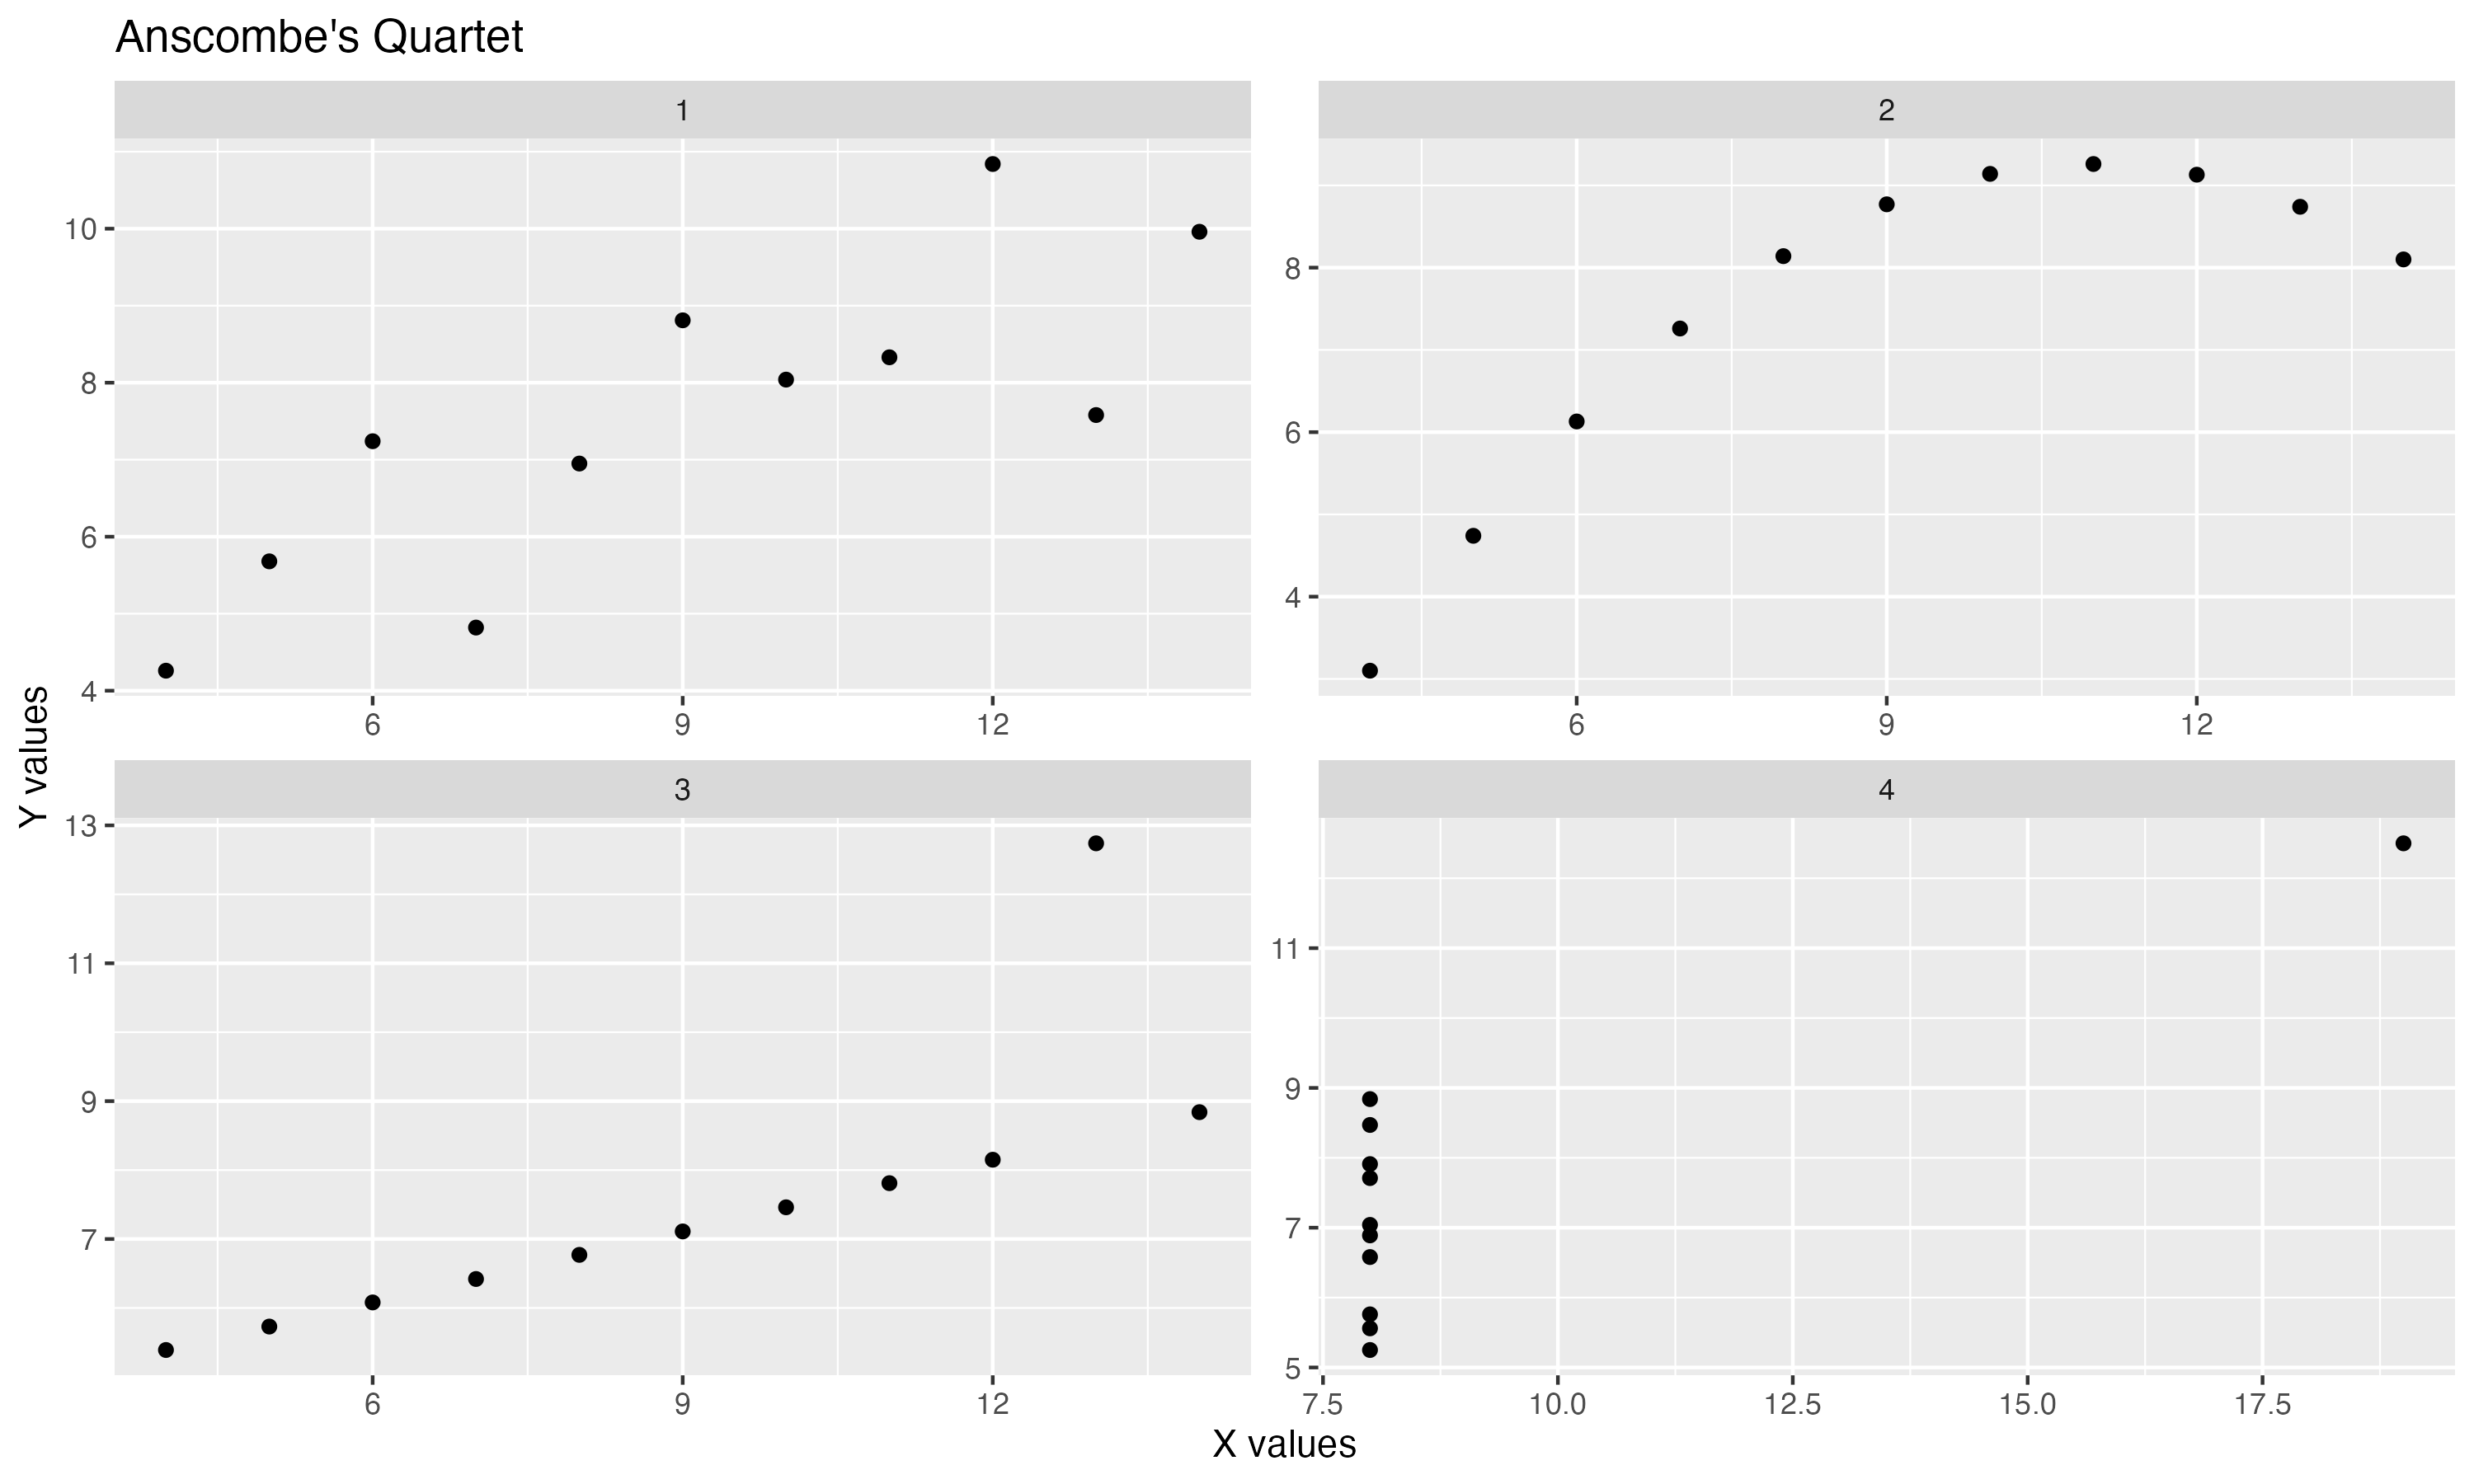
\includegraphics[width=0.9\textwidth]{../results/anscombe_quartet.png}
    \caption{Anscombe's Quartet}
    \label{fig:anscombe_quartet}
\end{figure}

\section{Fit a linear model to each dataset}

\lipsum[1-2]

% latex table generated in R 4.4.1 by xtable 1.8-4 package
% Sun Mar  9 16:15:36 2025
\begin{table}
    \centering
    \begin{tabular}{llrrrr}
      \hline
    model & term & coefficients & std\_errors & t\_values & p\_values \\ 
      \hline
    \multirow{2}{*}{data 1} & $\beta_0$ & 3.00 & 1.12 & 2.67 & 0.03 \\ 
      & $\beta_1$ & 0.50 & 0.12 & 4.24 & 0.00 \\ 
      \hline
    \multirow{2}{*}{data 2} & $\beta_0$ & 3.00 & 1.13 & 2.67 & 0.03 \\ 
      & $\beta_1$ & 0.50 & 0.12 & 4.24 & 0.00 \\ 
      \hline
    \multirow{2}{*}{data 3} & $\beta_0$ & 3.00 & 1.12 & 2.67 & 0.03 \\ 
      & $\beta_1$ & 0.50 & 0.12 & 4.24 & 0.00 \\ 
      \hline
    \multirow{2}{*}{data 4} & $\beta_0$ & 3.00 & 1.12 & 2.67 & 0.03 \\ 
      & $\beta_1$ & 0.50 & 0.12 & 4.24 & 0.00 \\ 
       \hline
    \end{tabular}
    \caption{Model Fitting Results} 
    \label{tab:model_fitting_results}
\end{table}

\begin{figure}[!h]
    \centering
    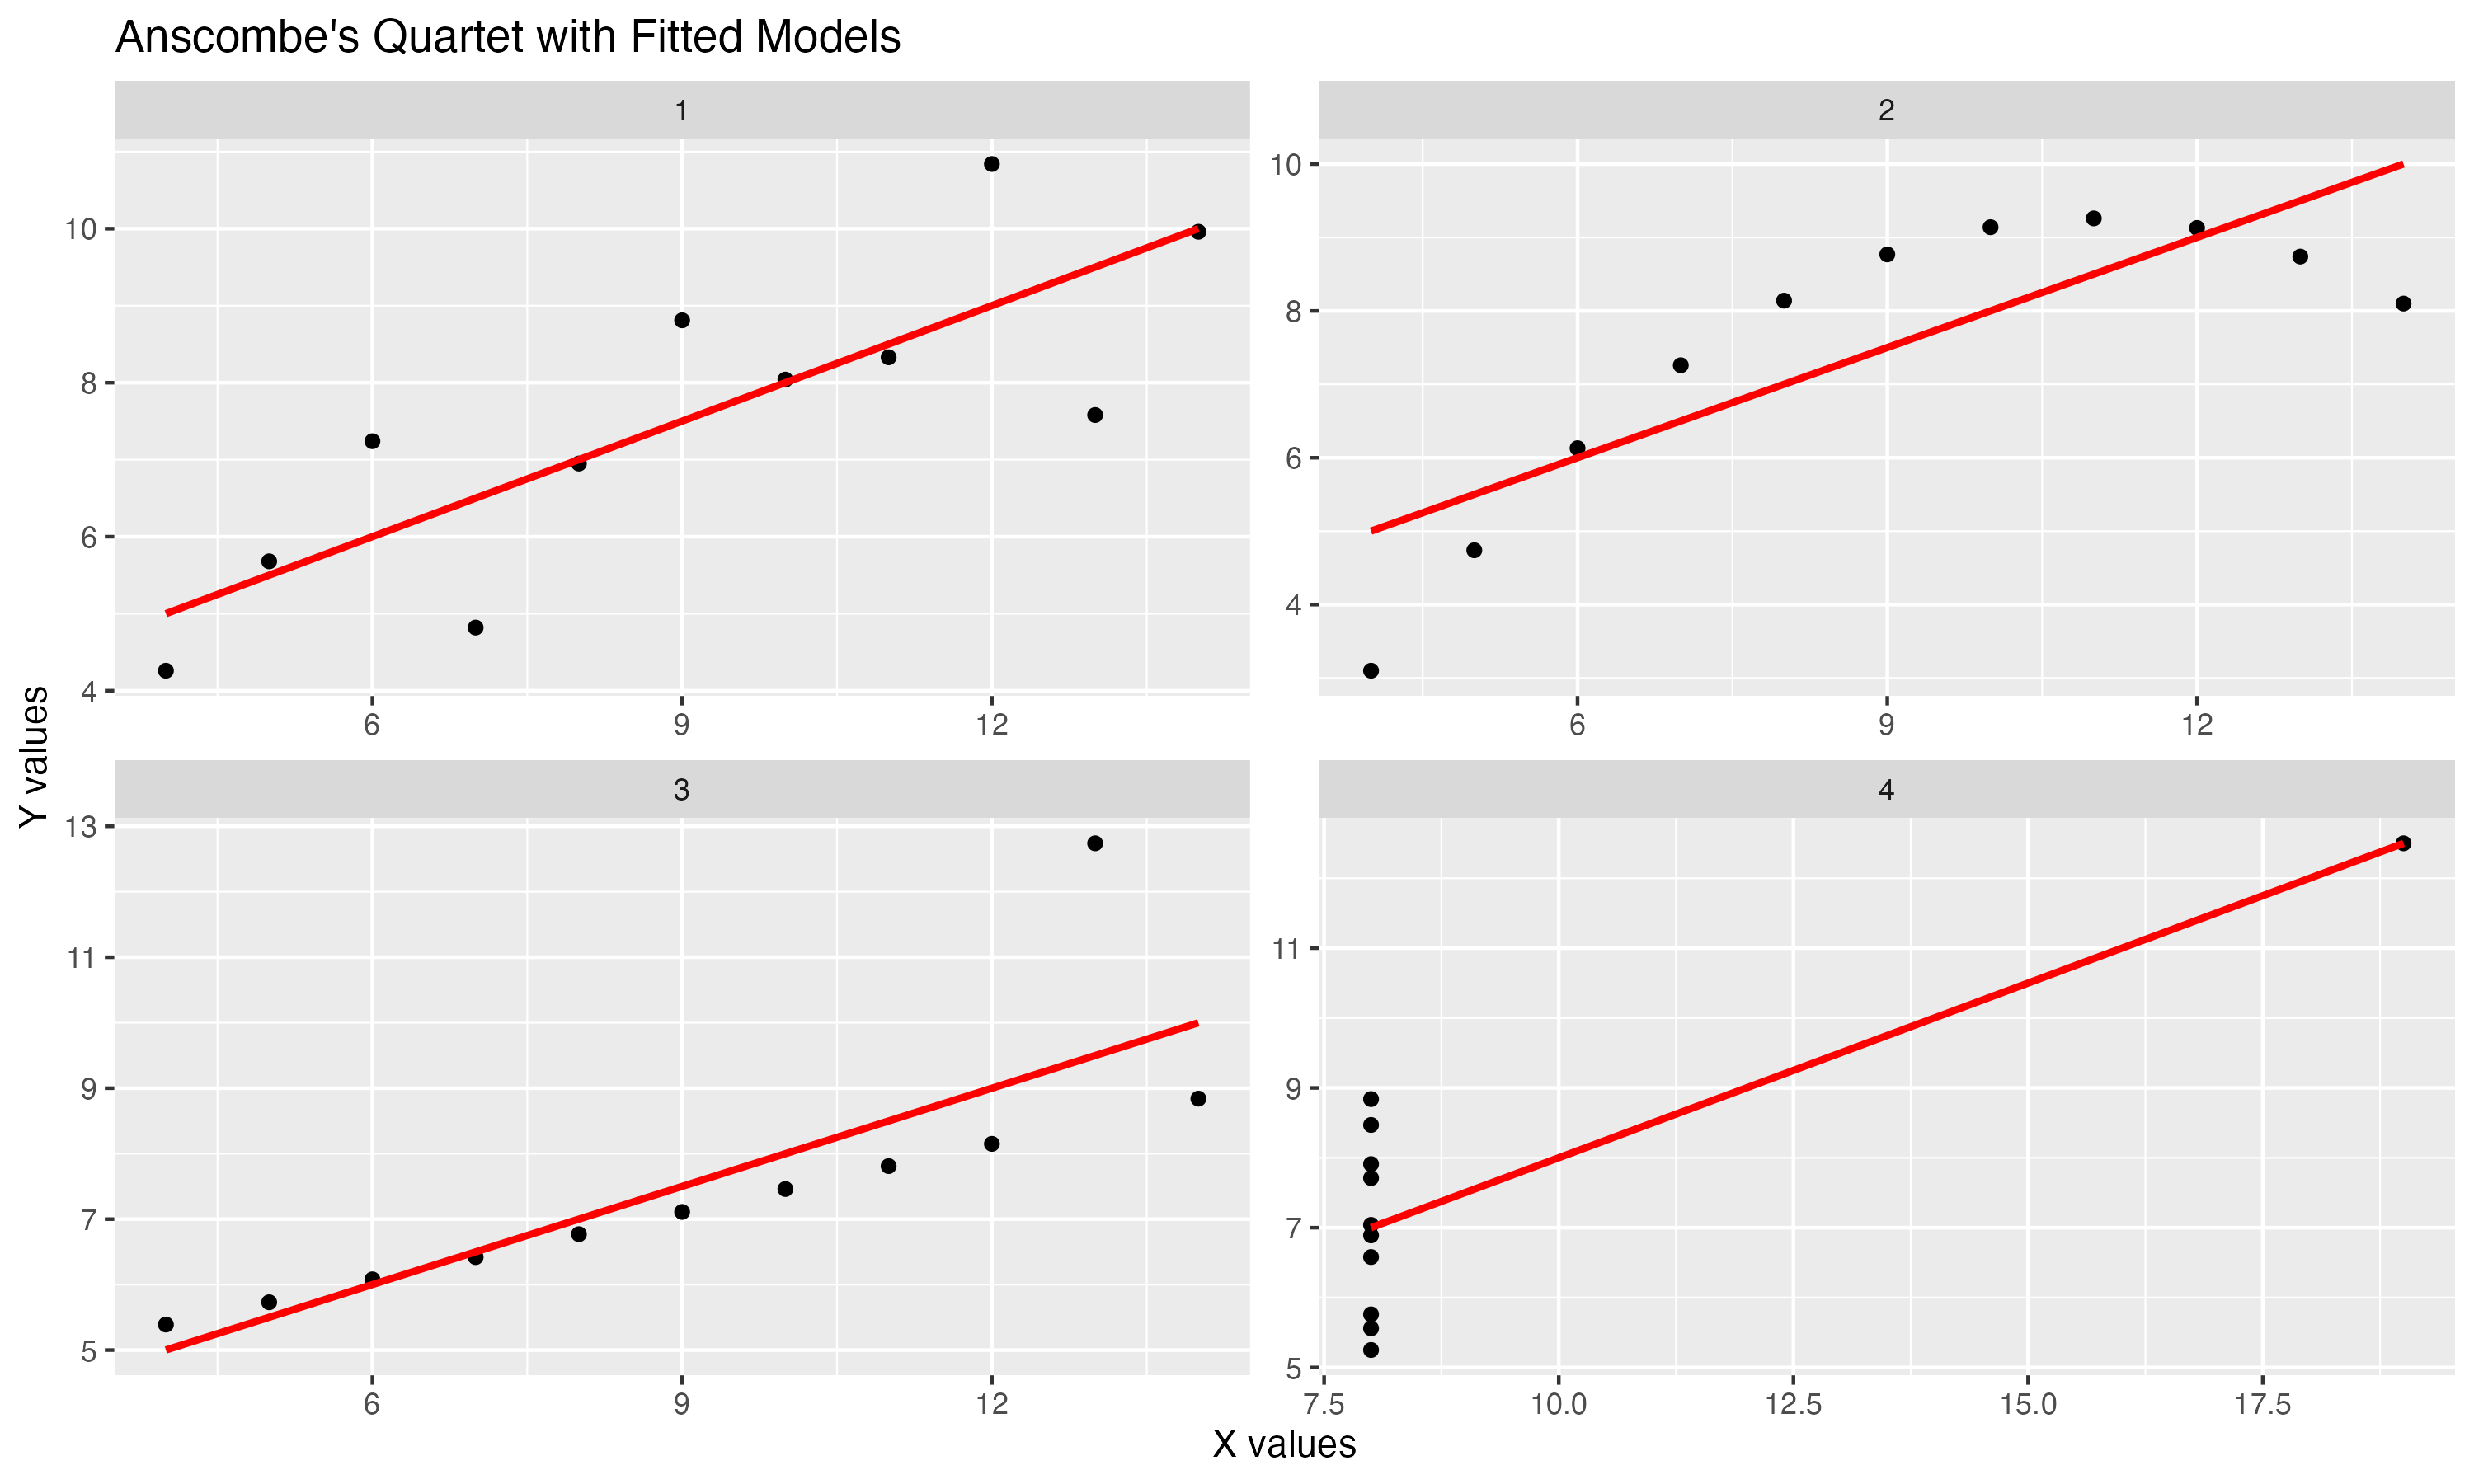
\includegraphics[width=0.9\textwidth]{../results/anscombe_quartet_fitted.png}
    \caption{Anscombe's Quartet with Fitted Lines}
    \label{fig:anscombe_quartet_fitted}
\end{figure}

\section{Residuals diagnostics}

\lipsum[1-2]


\begin{figure}[!h]
    \centering
    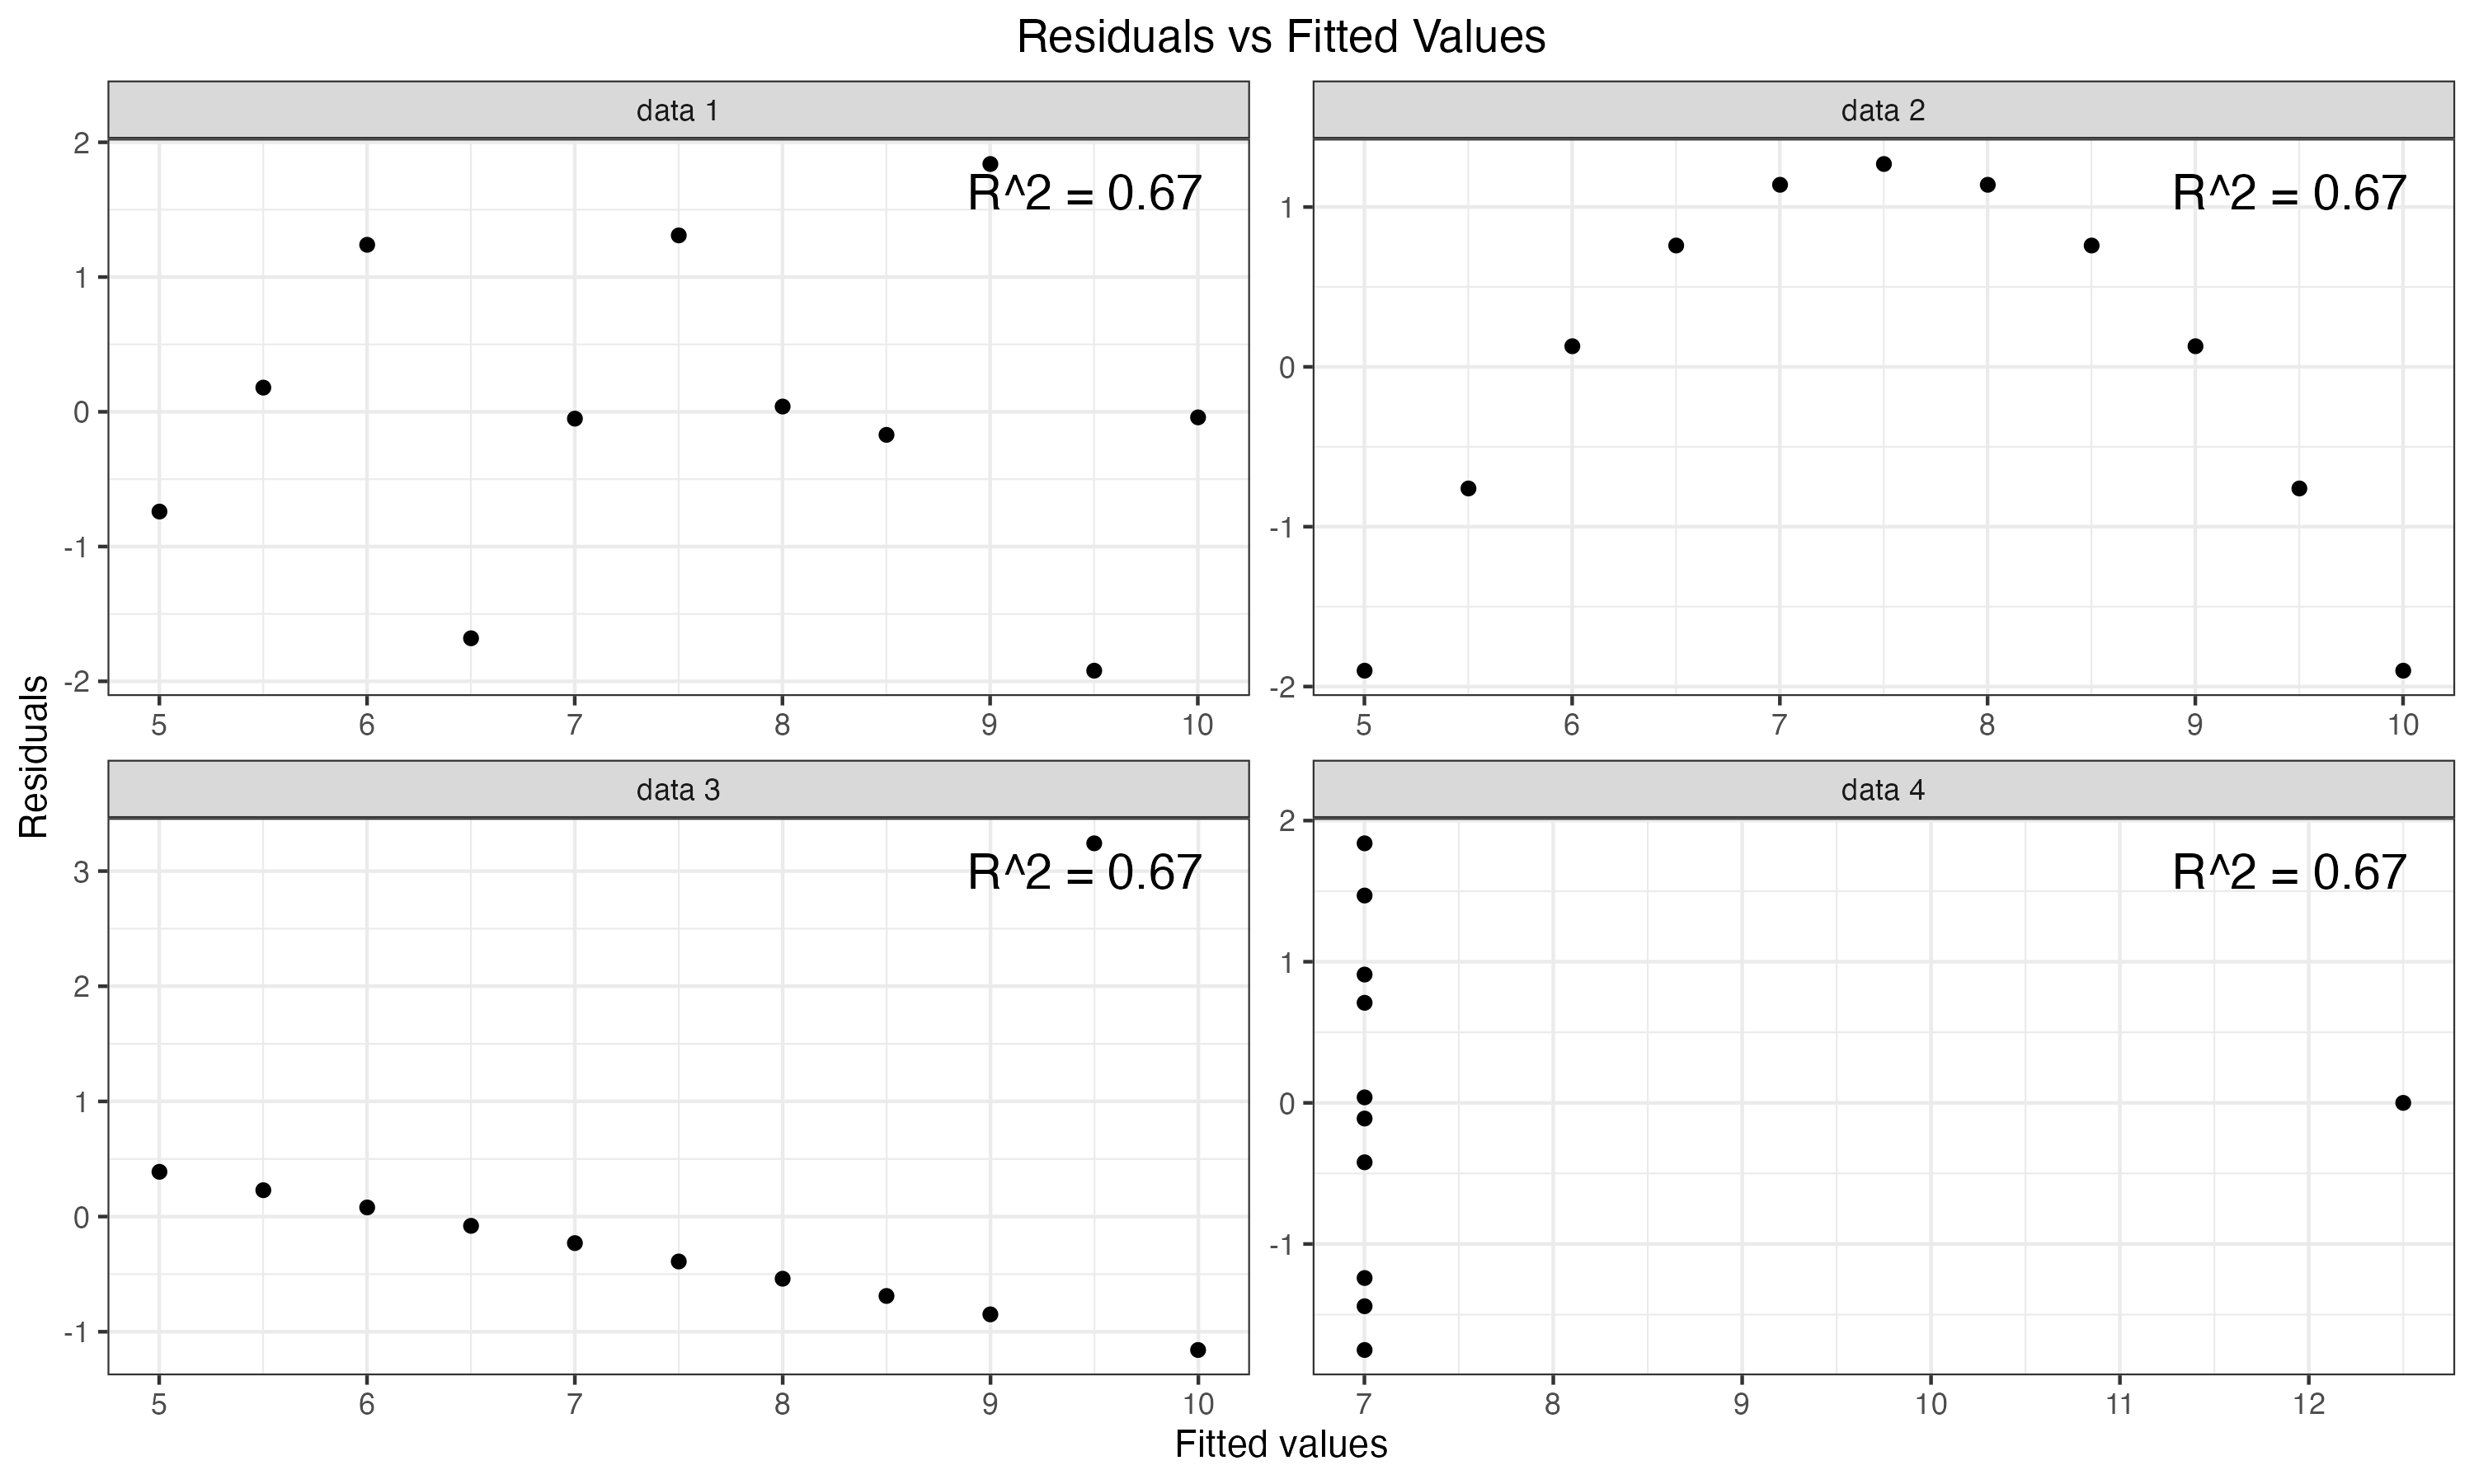
\includegraphics[width=0.9\textwidth]{../results/residuals_vs_fitted.png}
    \caption{Residuals vs Fitted Values}
    \label{fig:residuals_vs_fitted}
\end{figure}

\begin{figure}[!h]
    \centering
    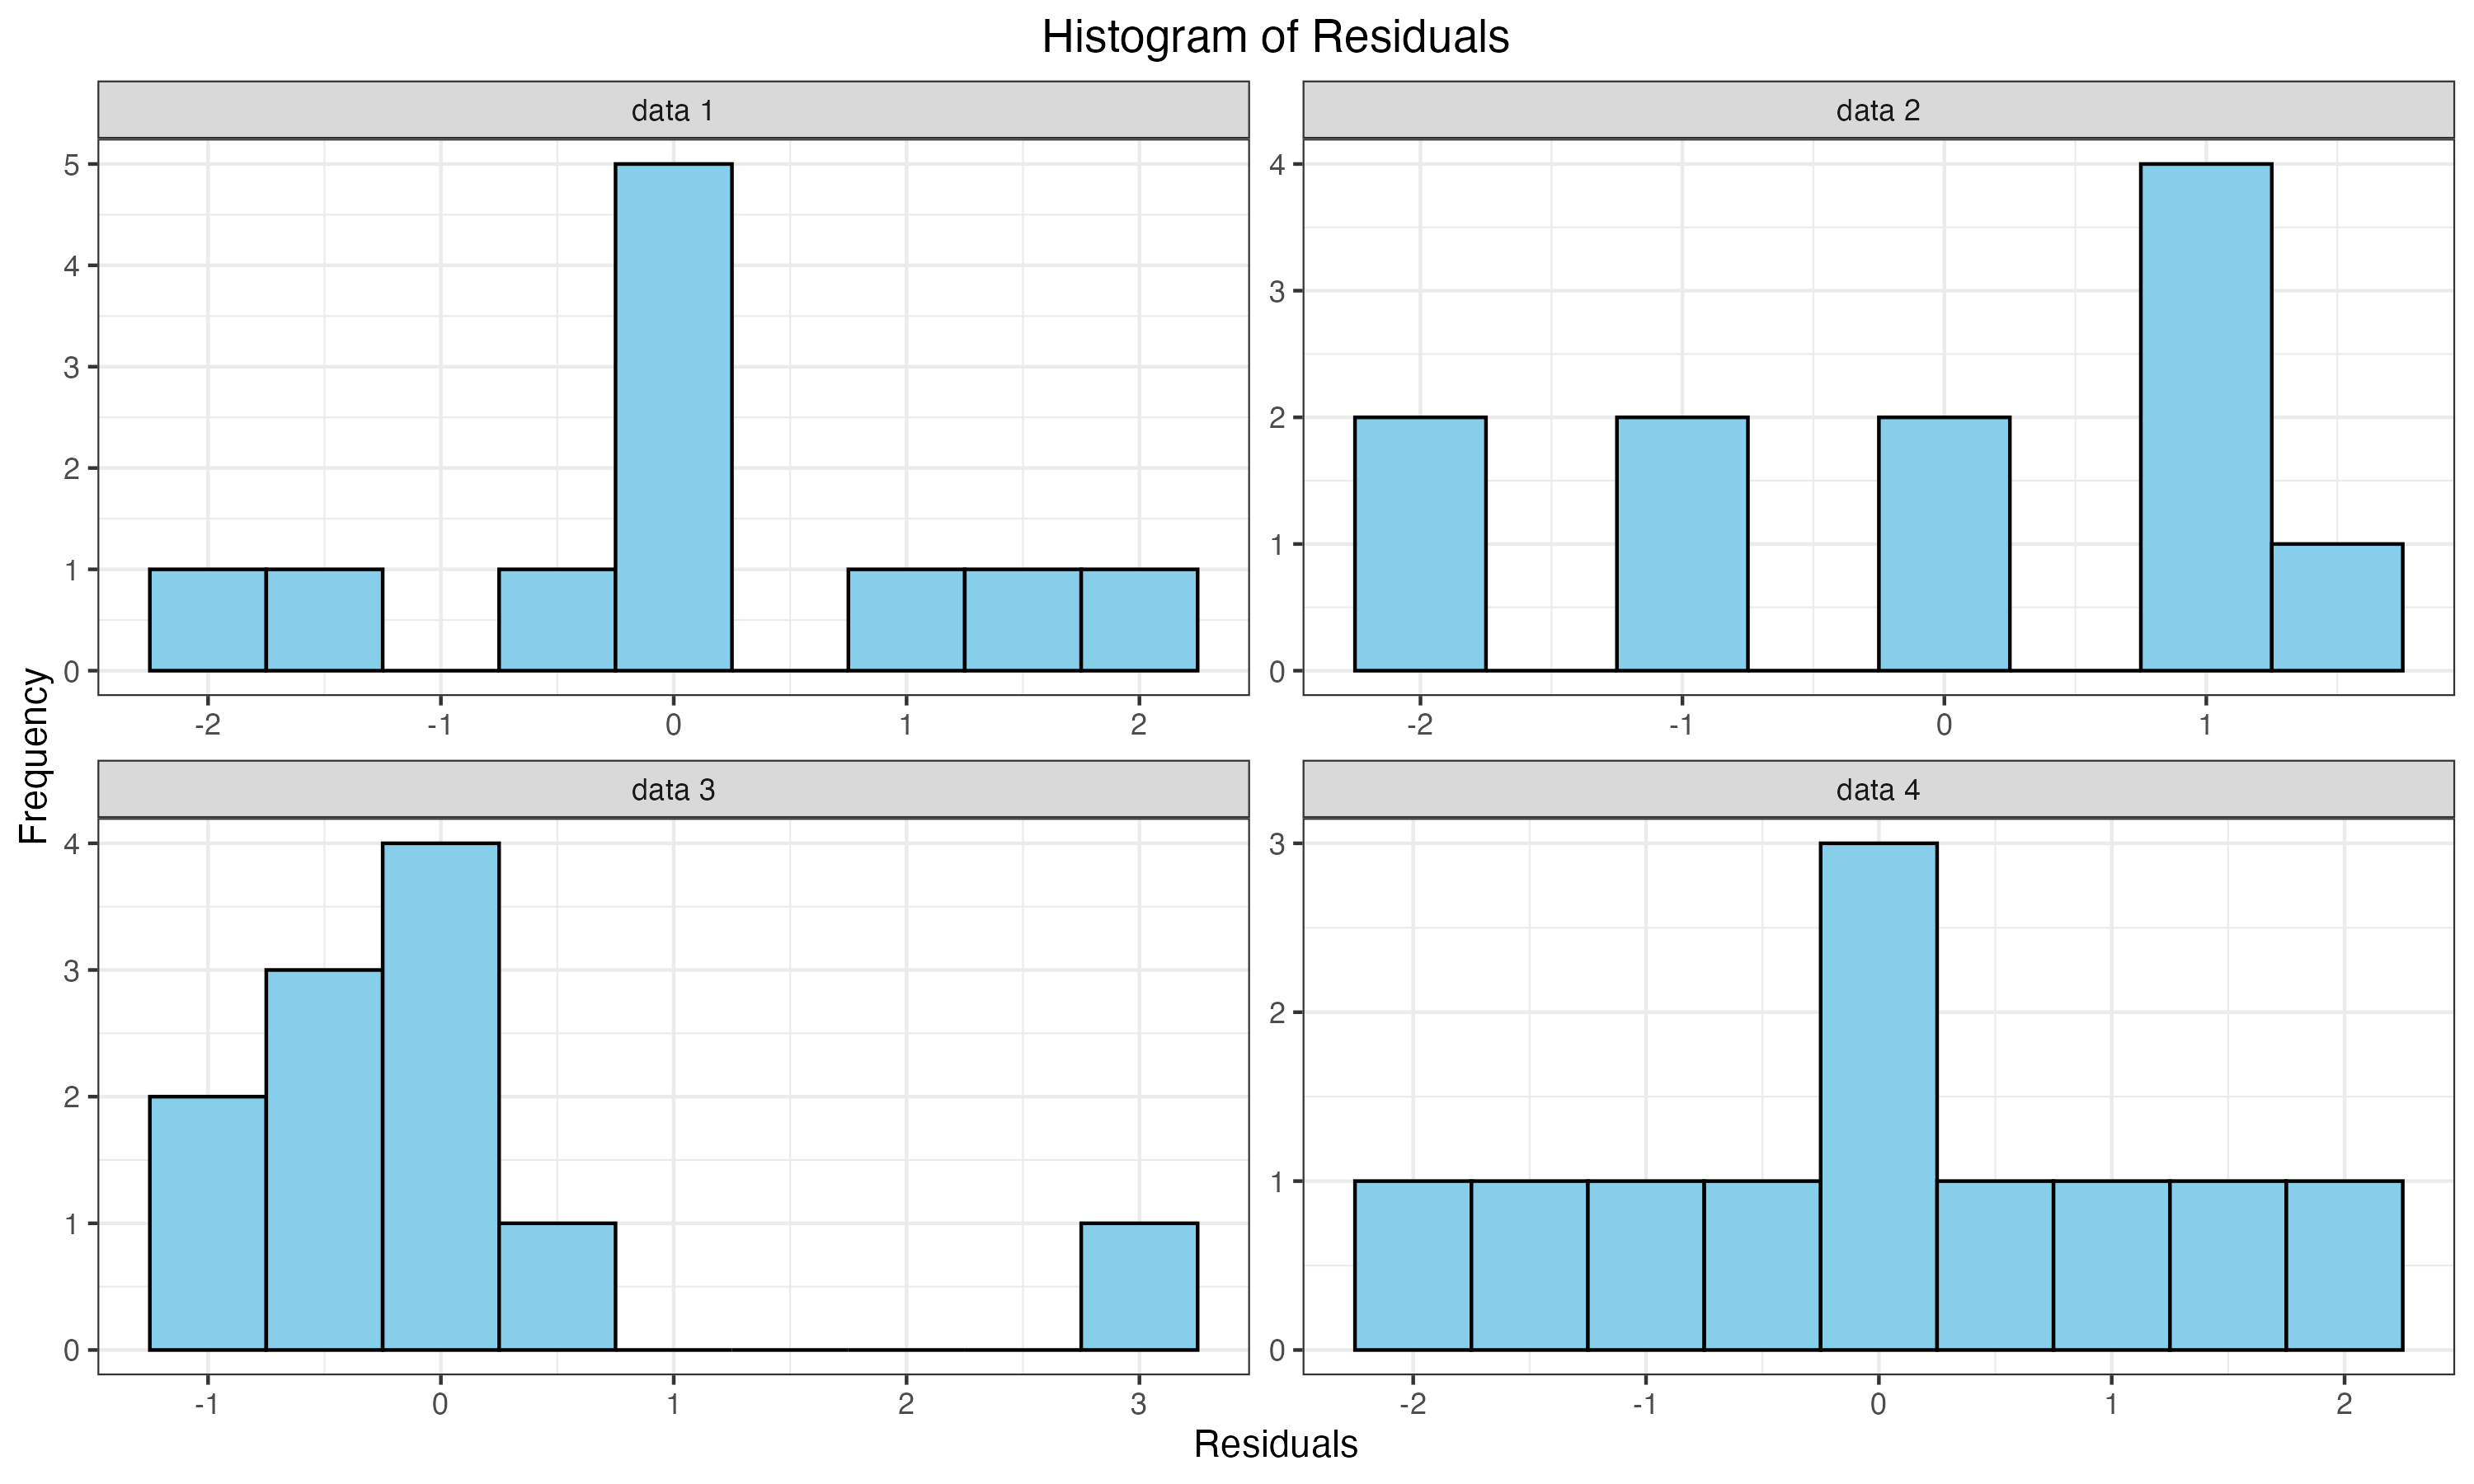
\includegraphics[width=0.9\textwidth]{../results/residuals_histogram.png}
    \caption{Histogram of Residuals}
    \label{fig:residuals_histogram}
\end{figure}

\begin{figure}
    \centering
    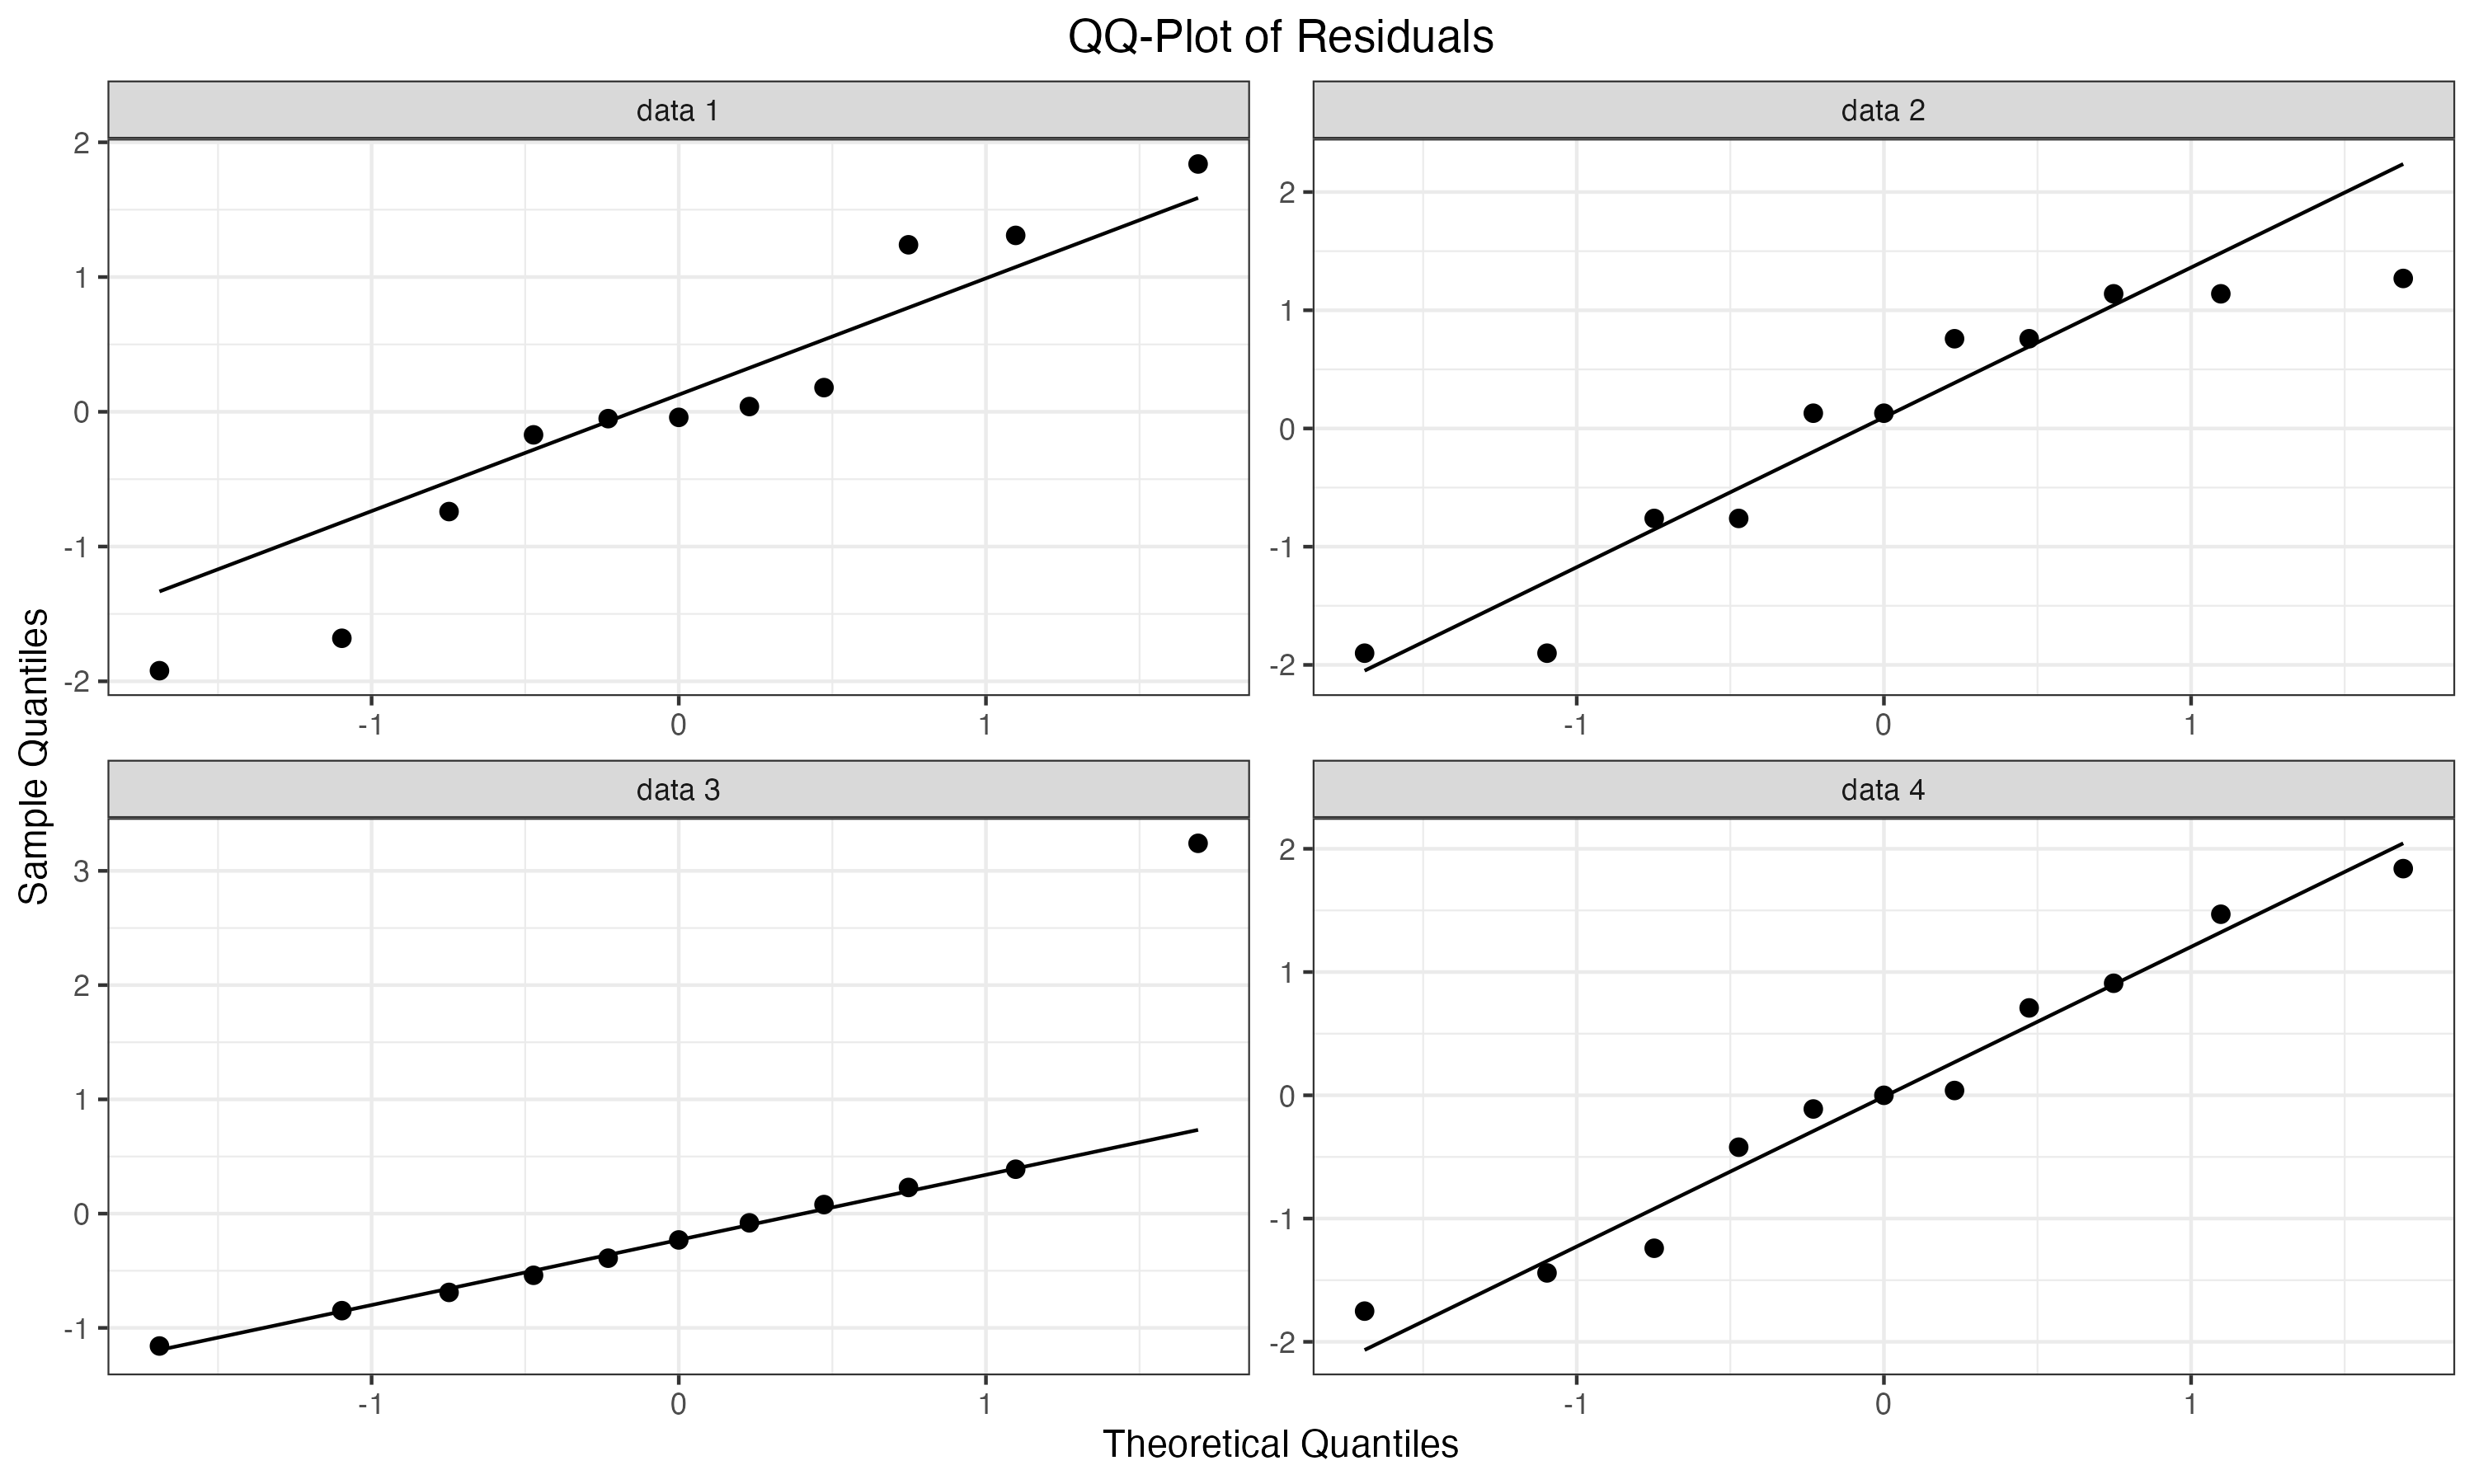
\includegraphics[width=0.9\textwidth]{../results/residuals_qq.png}
    \caption{Q-Q Plot of Residuals}
    \label{fig:residuals_qq}
\end{figure}



\clearpage
% Bibliography section
\begin{thebibliography}{99} % The number specifies the width of the label

  \bibitem{example1}
  H. Hyndman and G. Athanasopoulos. 
  ``STL Decomposition,'' 
  \textit{Forecasting: Principles and Practice (3rd ed.)}. 
  Available at: \url{https://otexts.com/fpp3/stl.html}. 
  Accessed: November 30, 2024.

\end{thebibliography}

\end{document}
